\documentclass[]{BasiliskReportMemo}

\newcommand{\submiterInstitute}{Autonomous Vehicle Simulation (AVS) Laboratory,\\ University of Colorado}

\newcommand{\ModuleName}{rwMotorVoltage}
\newcommand{\subject}{Mapping Reaction Wheel Motor Torques Commands to Servo Voltages}
\newcommand{\status}{Initial document draft}
\newcommand{\preparer}{H. Schaub}
\newcommand{\summary}{This FSW module takes a set of $N$ RW motor torques $\bm u_{s}$ and maps them into a set of RW servo voltages.  This modules has an open-loop mode that ensures the output voltage is between a minimum and maximum voltage magnitude using a linear mapping.  If the RW availability message is set, then then only the AVAILABLE RW voltages are computed.  The other are set to zero.  If the RW wheel speed message is available, then the torque control loop is engaged where a proportional control is used to track the desired torque value.  }


\begin{document}


\makeCover


%
%	enter the revision documentation here
%	to add more lines, copy the table entry and the \hline, and paste after the current entry.
%
\pagestyle{empty}
{\renewcommand{\arraystretch}{1.1}
\noindent
\begin{longtable}{|p{0.5in}|p{4.5in}|p{1.14in}|}
\hline
{\bfseries Rev}: & {\bfseries Change Description} & {\bfseries By} \\
\hline
v1.0 & Initial Document & H. Schaub \\
\hline

\end{longtable}
}

\newpage
\setcounter{page}{1}
\pagestyle{fancy}

\tableofcontents
~\\ \hrule ~\\


\section{Introduction}
There two types of RW control torque interfaces, analog and digital. This modules assumes the RW is controlled through a set of voltages sent to the RW motors.  This modules is developed in a general manner where a voltage deadband is assumed and the module can be run in a pure open-loop manner, or with a closed-loop torque tracking control mode.  Finally, if a RW availability message is present, then the RW is set to zero if the corresponding availability is set to {\tt UNAVAILABLE}. 



\begin{figure}[htb]
	\centerline{
	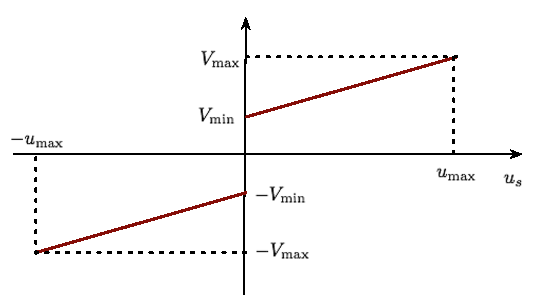
\includegraphics[]{Figures/us2V}
	}
	\caption{Illustration of RW motor torque to voltage conversion}
	\label{fig:us2V}
\end{figure}
\section{Open-loop voltage conversion}
this module requires the RW configuration message to contain the maximum RW motor torque values $u_{\text{max}}$.  The user must specify the minimum and maximum output voltages as shown in Figure~\ref{fig:us2V}.  The minimum voltage is a voltage below which the motor doesn't apply a torque, i.e. a deadzone.  

Let the intermediate voltage value $V_{\text{int}}$ as
\begin{equation}
	\label{eq:rwMV:1}
	V_{\text{int}} = \frac{V_{\text{max}} - V_{\text{min}}}{u_{\text{max}}} u_{s}
\end{equation}
The output voltage is thus determined through
\begin{equation}
	V = V_{\text{int}} + V_{\text{min}} *\text{sgn}(V_{\text{int}} )
\end{equation}

\section{RW Availability} 
If the input message name {\tt rwAvailInMsgName} is defined, then the RW availability message is read in. The voltage mapping is only performed if the individual RW availability setting is {\tt AVAILABLE}.  If it is {\tt UNAVAILABLE} then the output voltage is set to zero.  


\section{Closed-loop commanded torque tracking}
The requested RW motor torque is given by $u_{s}$.  The RW wheel speed $\Omega$ is monitored to see if the actual torque being applied matches the commanded torque.  Let $J_{s}$ be the RW spin inertia about the RW spin axis $\hat{\bm g}_{s}$.   In the following development the motor torque equation is approximated as
\begin{equation}
	u_{s} = J_{s} \dot\Omega
\end{equation}
where the assumption is made that the spacecraft angular accelerations are small compared to the RW angular accelerations.  The $\dot\Omega$ term is digitally evaluated using a backwards difference method:
\begin{equation}
	\dot\Omega_{n} = \frac{\Omega_{n} - \Omega_{n-1}}{\Delta t}
\end{equation}
Care is taken that the old RW speed information $\Omega_{n-1}$ is not used unless a history of wheel speeds is available, in particularly after a module reset.  Thus, the actual RW torque is evaluated as
\begin{equation}
	u_{n} = J_{s} \dot\Omega_{n}
\end{equation}
Finally, the closed loop motor torque value is computed with a proportional feedback component as
\begin{equation}
	u_{s,CL} = u_{s} - K (u_{n} - u_{s})
\end{equation}
where $K>0$ is a positive feedback gain value.  Finally, this $u_{s,CL}$ is fed to the voltage conversion process in Eq.~\eqref{eq:rwMV:1}.  




\section{Unit Test Discussion}
A series of unit tests are performed to check the validity of this module's operation.

\subsection{Test 1}
The first test uses an input vector of \input{AutoTex/usFalseFalseFalse.tex} Nm.  The RW spin inertia is set to $J_{s}$ = 0.1 kg m$^{s}$, while the maximum RW motor torque is set to $u_{\text{max}}$ = 0.2 Nm.  In this test case no RW availability or wheel speed messages are set.  The simulation is first run for 1.5 seconds with a 0.5 second control update period.  Next, the module is reset and run for another 1.5 sections.  With only the open-loop voltage conversion active and the RW motor torque
The resulting actual values and differences with hand-computed values are shown in Table~\ref{tbl:testFalseFalseFalse}.  The reset of the module should have not impact on the voltage conversion, which is the case.

\input{AutoTeX/testFalseFalseFalse.tex}

\subsection{Test 2}
This test repeats the values of test 1, except that the RW motor torque input vector is set to \input{AutoTex/usTrueFalseFalse.tex} Nm.  This should saturated the first and last RW voltage output, which is seen in Table~\ref{tbl:testTrueFalseFalse}. 

\input{AutoTeX/testTrueFalseFalse.tex}

\subsection{Test 3}
This test repeats the values of test 1, except that a RW availability message is created.  Here all RWs have a status of {\tt AVAILABLE} except for the 3rd RW which is {\tt UNAVAILALBE}.    The 3rd RW voltages should thus all be 0.0 in this case, which is seen in Table~\ref{tbl:testFalseTrueFalse}. 

\input{AutoTeX/testFalseTrueFalse.tex}

\subsection{Test 4}

This test repeats the values of test 1, except that a RW wheel speed message is created.  The feedback gain is set to $K = 1.5$.  For the first 1.0 seconds the RW wheel speeds are set to \input{AutoTeX/Omega1.tex} rad/sec.  At 1.0 seconds the RW wheel speeds are set to  \input{AutoTeX/Omega2.tex} rad/sec.  Then the module is reset at 1.5 seconds and the simulation continued for another 1.5 second for a 3 second total simulation time.   The speed message remains the same after the reset.   Table~\ref{tbl:testFalseFalseTrue} shows the results of the actual values, and the differences with the hand-computed values.  

\input{AutoTeX/testFalseFalseTrue.tex}




\end{document}
